\chapter{Methodology}

\section{System Architecture}

The overall system is designed to automatically search for a resource-efficient convolutional neural network (CNN) architecture and deploy it on a microcontroller. Figure~\ref{fig:architectural_pipeline} outlines the methodology pipeline, which consists of the following stages: 

\begin{enumerate}
    \item Defining a flexible model architecture and search space,
    \item Training and evaluating candidate models (including profiling their resource usage),
    \item An evolutionary search loop (Neural Architecture Search) driven by a genetic algorithm with a surrogate model, and
    \item Model export and deployment to the embedded device.
\end{enumerate}

Each stage is described below.

\begin{figure}[ht]
    \centering
    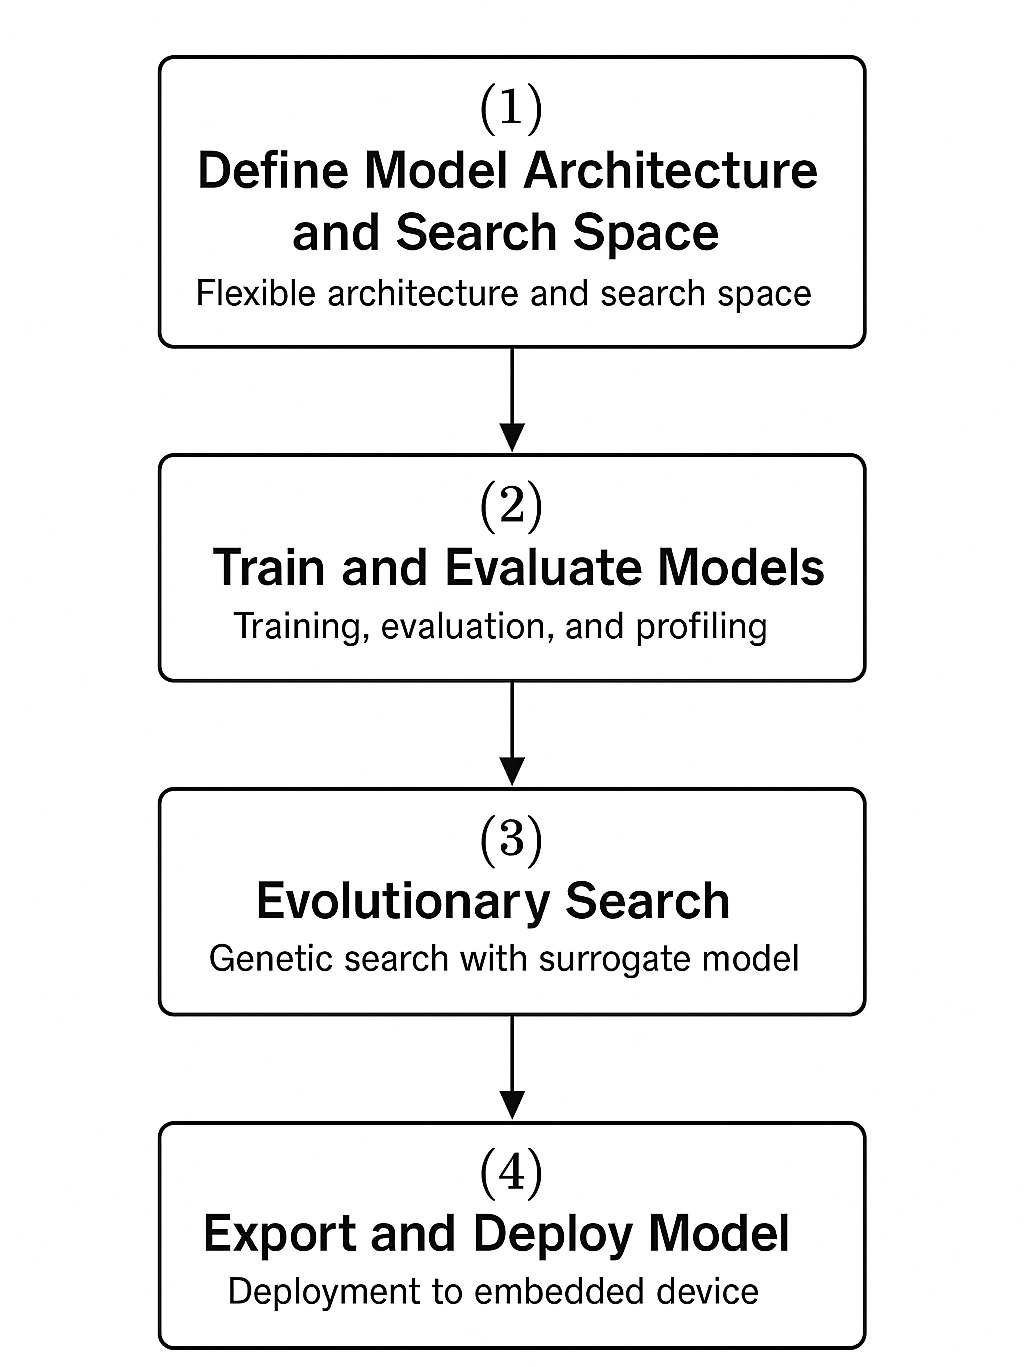
\includegraphics[width=0.6\linewidth]{Pictures/Architegture.png}
    \caption{Architectural pipeline}
    \label{fig:architectural_pipeline}
\end{figure}

\subsection*{Model Creation}

We developed a custom model class \texttt{TakuNetModel} that can construct CNNs from a set of architecture parameters. These parameters (drawn from a predefined search space) define the network’s configuration (e.g., number of layers, kernel sizes etc.). The model is assembled modularly: an initial stem block processes the input, followed by a sequence of repeated stage blocks, and ending with a refiner block that produces the final classification output.

This design allows different architectures to be instantiated by simply varying a configuration dictionary. More about this architecture and the reason it is selected will be explained in the \hyperref[chap:Architecture]{relevant chapter}.


\subsection*{Training and Evaluation}



The training and evaluation phase is a critical part of the overall pipeline, responsible for assessing the performance and efficiency of each candidate CNN architecture generated during the Neural Architecture Search (NAS) process. The primary goal is to determine how well each model performs not only in terms of classification accuracy, but also in terms of its resource consumption, making it suitable for deployment on resource-constrained microcontrollers.

\begin{enumerate}

    \item \textbf{Dataset CIFAR-100}
    
    All models are trained and evaluated using the CIFAR-100 dataset which consists of:
\begin{itemize}
    \item 60,000 color images of size 32x32 pixels
    \item 100 distinct classes (600 images per class)
\item a standard split: 50,000 training images and 10,000 test images

\end{itemize}
The dataset is challenging due to its high number of classes and imbalanced class distribution, which increases the importance of using evaluation metrics beyond just accuracy.

    \item \textbf{Model Training}
    Each candidate architecture is trained from scratch using TensorFlow 2.18.0, with GPU acceleration enabled where available. The training pipeline includes the following steps:
    
\begin{itemize}
    \item \textbf{Initialization:} Models are initialized and built dynamically based on sampled architecture parameters from the search space.
    \item \textbf{Training Metrics:} \textit{Training Accuracy} is recorded per epoch to monitor learning progress and \textit{Validation Accuracy} is used to estimate generalization and prevent overfitting.

\end{itemize}

Training is kept consistent across models to ensure fair comparison in the NAS loop.
\item \textbf{Post-Training Evaluation}

After training, each model is evaluated on the test set using several key performance metrics: 
\begin{itemize}
    \item \textbf{Test Accuracy}: Overall classification accuracy across all test images.
    \item \textbf{Precision}: The proportion of correct positive predictions per class.
    \item \textbf{Recall}: The proportion of actual positives that were correctly identified.
    \item \textbf{F1-Score}: The harmonic mean of precision and recall, particularly useful for imbalanced datasets like CIFAR-100.


\end{itemize}

These metrics provide a more comprehensive understanding of model performance, especially for classes with fewer training examples.

\item \textbf{Resource Profiling}

In addition to classification performance, the system profiles the model’s resource consumption, which is crucial for microcontroller deployment:
\begin{itemize}
    \item \textbf{RAM Usage}: Peak memory usage during inference.
    \item \textbf{Flash/ROM Usage}: Total size of the model when serialized and stored.
    \item \textbf{Wall-clock Training Time}: Total time taken for training, useful for tuning NAS runtime.
\end{itemize}

These metrics are essential for multi-objective optimization, where the aim is to balance accuracy with hardware constraints.
\item \textbf{Purpose}

The training and evaluation phase serves a dual purpose:
\begin{itemize}
    \item To \textbf{quantify model performance} using standard machine learning metrics, ensuring the model is suitable for the classification task.
    \item To\textbf{ assess the resource efficiency }of each architecture, which is necessary for identifying models that can be deployed on low-power embedded devices.
\end{itemize}

The output of this phase—accuracy metrics and resource profiles—is fed into the evolutionary search loop, where it helps guide the selection and evolution of more optimal architectures in subsequent generations.


    
\end{enumerate}




\subsection{NAS Evolutionary Loop}

To automate the discovery of high-performing neural network architectures, we use a \textbf{genetic algorithm} — a technique inspired by the process of natural selection. This approach allows us to explore a large space of possible model architectures without manually designing each one.

The process is organized around a population of candidate models, which evolves over time. The goal is to \textbf{optimize a fitness function} that takes into account both the model’s \textbf{accuracy} and its \textbf{resource usage} (such as memory, number of parameters, or inference time).
Here is a breakdown of how this process works:

\textbf{Initial Population Sampling}
\begin{itemize}
    \item We start by randomly generating an initial set of architectures from the defined search space.
    \item Each architecture represents a different neural network design, with varying numbers of layers, filter sizes, activation functions, etc.
    \item These models form the first generation of the population.


\end{itemize}

\textbf{Evolutionary Loop (Repeated for Several Generations)}

In each generation, the population is updated through three main steps:
\begin{enumerate}
    \item \textbf{Parent Selection}
    \begin{itemize}
        \item From the current population, we select a group of promising models that have performed well according to the fitness function.
        \item We use tournament selection, where a small group of models is randomly chosen, and the best among them is selected as a parent.
        \item This ensures that stronger candidates are more likely to pass on their characteristics to the next generation, while still maintaining diversity.
    \end{itemize}
    \item \textbf{Crossover}
    \begin{itemize}
        \item Selected parent models are recombined to produce new architectures, known as offspring.
        \item This process combines parts of two or more parent architectures, similar to genetic recombination in biology.
        \item The idea is to inherit beneficial traits from different models and explore new combinations.


    \end{itemize}
    \item \textbf{Mutation}
    \begin{itemize}
        \item To introduce variation and novelty, some parts of the offspring architectures are randomly modified.
        \item This could mean changing a layer’s type, adjusting filter size, altering the number of neurons, or modifying other hyperparameters.
        \item Mutation helps prevent the population from converging too early to suboptimal solutions.


    \end{itemize}
\end{enumerate}
  
\textbf{Termination Strategy and Output}

The NAS process is executed for a fixed duration of 5 hours. During this time, all trained models are collected and stored for further analysis. At the end of the search, the algorithm returns the final \textit{Pareto front}, which includes all non-dominated architectures that offer optimal trade-offs between competing objectives—such as accuracy, memory usage, and flash size. These Pareto-optimal models represent the best candidates discovered within the given time budget.

This evolutionary process allows us to discover well-balanced and efficient neural architectures without manual trial and error. It is especially useful in scenarios where both performance and efficiency are critical.




\section{Hardware and Software Tools}

Our methodology relies on a combination of software frameworks for machine learning and a target embedded hardware platform. We describe the tools and platforms used below.

\subsection*{TensorFlow and Keras}

We built and trained all neural networks using TensorFlow (version 2.x) with the Keras API. The \texttt{TakuNetModel} class is a Keras \texttt{Model} under the hood, composed of standard Keras layers such as \texttt{Conv2D}, \texttt{DepthwiseConv2D}, and \texttt{Dense}. This choice provided high-level flexibility in defining arbitrary model architectures.

Training was performed on a workstation with GPU support, The GPU used in our experiments was the \textbf{Tesla V100 SXM2 32GB}.
In addition, we used auxiliary Python libraries: \texttt{scikit-learn} for computing evaluation metrics (precision, recall, F1-score), and \texttt{pandas} for logging results. The genetic algorithm are also implemented in Python using \texttt{NumPy} and \texttt{TensorFlow}. This entire experimentation framework runs offline on a PC.

\subsection*{TensorFlow Lite for Microcontrollers}

To bridge the gap between PC-trained models and deployment on a microcontroller, we used TensorFlow Lite. Specifically, trained models were converted to the TensorFlow Lite FlatBuffer format, and then deployed using TensorFlow Lite for Microcontrollers (TFLite Micro).

TFLite Micro is a lightweight inference engine designed for memory-limited devices. It supports a subset of TensorFlow operators, which influenced our model design to use only supported ops. After training a model in Keras, we used the TFLite converter to produce a quantized \texttt{.tflite} model.

We then developed a utility to convert this binary model into a C array stored in a \texttt{.h} header file. The following Python code illustrates this process:

\begin{lstlisting}[language=Python, caption={Convert a TFLite model to a C header array for Arduino deployment}, label=lst:tflite_to_c_array]
# Convert tflite model to C array for Arduino
with open(f"{self.model_name}.tflite", "rb") as f:
    tflite_bytes = f.read()
c_array = ", ".join(f"0x{b:02x}" for b in tflite_bytes)
model_length = len(tflite_bytes)
header_content = (
    f"#ifndef {self.model_name.upper()}_H\n#define {self.model_name.upper()}_H\n\n"
    f"const unsigned char {self.model_name}_data[{model_length}] = {\n    {c_array}\n}};\n"
    f"const unsigned int {self.model_name}_length = {model_length};\n\n#endif"
)
with open(f"{self.model_name}.h", "w") as header_file:
    header_file.write(header_content)
\end{lstlisting}

This header defines two symbols: an array of bytes with the model data, and a variable with its length. This header is then included in the Arduino project.

On the Arduino side, we use the official TensorFlow Lite Micro library (available through the Arduino Library Manager). The process involves:

\begin{itemize}
    \item Allocating a memory arena (an array of bytes) for use by the TFLite Micro runtime.
    \item Initializing the model interpreter with the model data and memory arena.
    \item Invoking inference on new input data using the interpreter.
\end{itemize}


As a targeted Hardware environment we choose \textbf{Arduino Nano 33 BLE Sense}. More on about the procedure of the deployment will be explain in the  \hyperref[chap:DeploymentEnvironment]{relevant chapter}.


